%------------------------
% Resume — PRINT version (no hyperlinks; for paper distribution)
% Source: Resume_en.tex with all \href{...}{...} stripped and Sources: lines removed.
% Original template:
% Author : Anubhav Singh
% Github : https://github.com/xprilion
% License : MIT
%------------------------

\documentclass[a4paper,20pt]{article}

\usepackage{latexsym}
\usepackage[empty]{fullpage}
\usepackage{titlesec}
\usepackage{marvosym}
\usepackage[usenames,dvipsnames]{color}
\usepackage{verbatim}
\usepackage{enumitem}
\usepackage[pdftex]{hyperref}
\usepackage{fancyhdr}
\usepackage{graphicx}
\usepackage{CJKutf8} % for occasional Chinese (e.g., patent original title)

\pagestyle{fancy}
\fancyhf{} % clear all header and footer fields
\fancyfoot{}
\renewcommand{\headrulewidth}{0pt}
\renewcommand{\footrulewidth}{0pt}

% Adjust margins
\addtolength{\oddsidemargin}{-0.530in}
\addtolength{\evensidemargin}{-0.375in}
\addtolength{\textwidth}{1in}
\addtolength{\topmargin}{-.45in}
\addtolength{\textheight}{1in}

\urlstyle{rm}

\raggedbottom
\raggedright
\setlength{\tabcolsep}{0in}

% Sections formatting
\titleformat{\section}{
  \vspace{-10pt}\scshape\raggedright\large
}{}{0em}{}[\color{black}\titlerule \vspace{-6pt}]

%-------------------------
% Custom commands
\newcommand{\resumeItem}[2]{
  \item\small{
    \textbf{#1}{#2}
  }
}

\newcommand{\resumeItemWithoutTitle}[1]{
  \item\small{
    {\vspace{-2pt}}
  }
}

\newcommand{\resumeSubheading}[5]{
  \item \textbf{#1}{\hfill #2} \\
        #3 \hfill #4 \\
        #5
}


\newcommand{\resumeSubItem}[2]{\resumeItem{#1}{#2}\vspace{-3pt}}

\renewcommand{\labelitemii}{$\circ$}

\newcommand{\resumeSubHeadingListStart}{\begin{itemize}[leftmargin=*]}
\newcommand{\resumeSubHeadingListEnd}{\end{itemize}}
\newcommand{\resumeItemListStart}{\begin{itemize}}
\newcommand{\resumeItemListEnd}{\end{itemize}\vspace{-5pt}}

%-----------------------------
%%%%%%  CV STARTS HERE  %%%%%%

\begin{document}

%----------HEADING-----------------
\begin{tabular*}{\textwidth}{l@{\extracolsep{\fill}}r}
\vspace{-50pt}
    \textbf{{\LARGE Yue Lin}} \\
    & 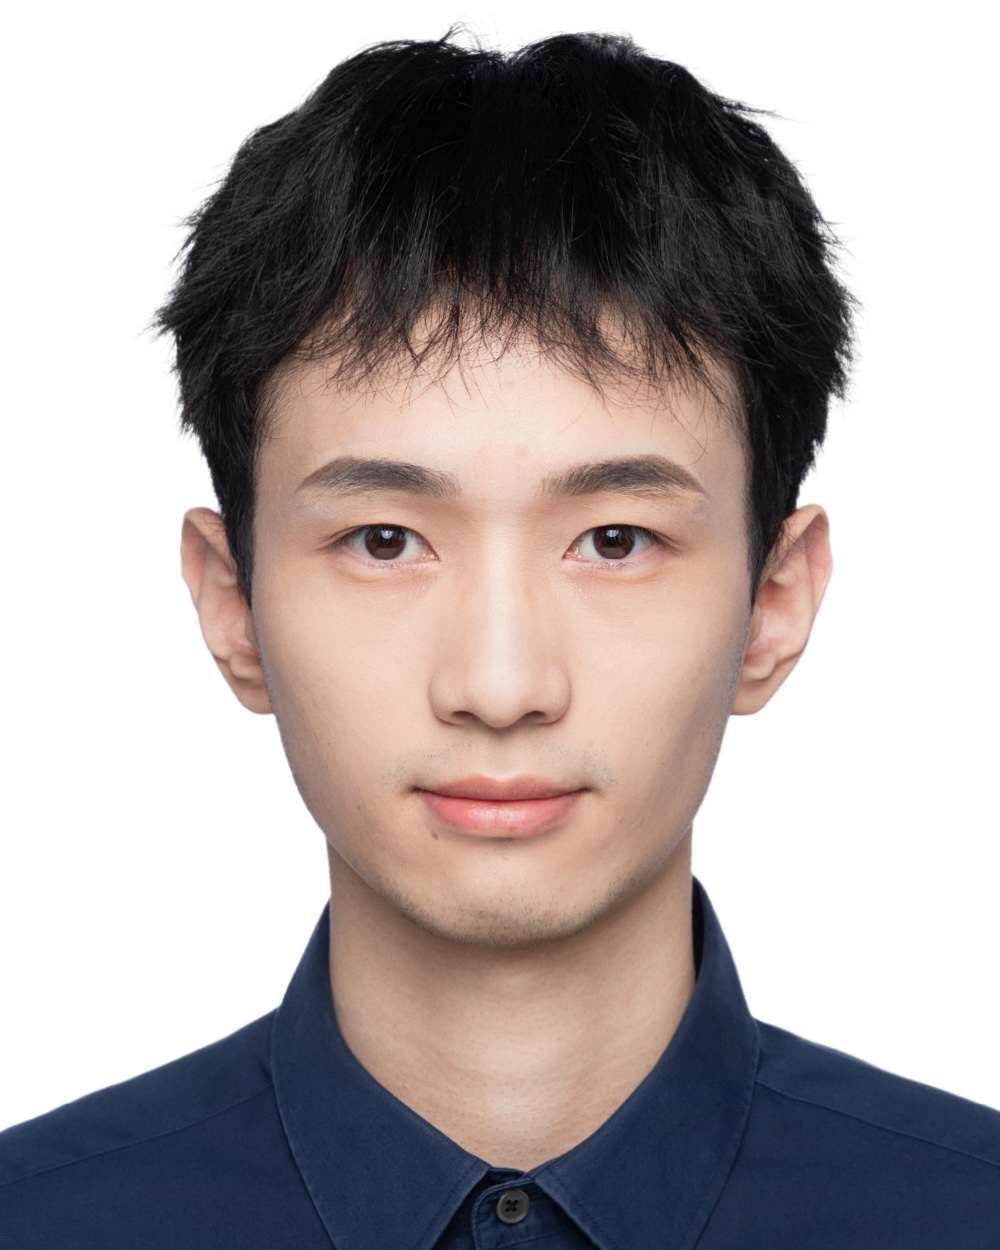
\includegraphics[width=0.1\linewidth]{ly2023white5_1cun.jpeg}\\
\vspace{-10pt} \\
    PhD Student, School of Data Science
    & Blog:~~~~~~yuelin301.github.io\\
    The Chinese University of Hong Kong, Shenzhen
    & Email:~linyue3h1@gmail.com \\
    & Mobile:~~~+86-187-5817-2219 \\
  % Github:  \\
\end{tabular*}

%-----------Education & Experience-----------------
\vspace{10pt}
\section{Education \& Experience}
\vspace{3pt}

\resumeSubHeadingListStart
    \resumeSubheading{The Chinese University of Hong Kong, Shenzhen}{Shenzhen, China}
    {\textit{PhD Student - School of Data Science}}{2024.8 - Present}
    {Research Interests: Multi-Agent Reinforcement Learning, Information Design.}
    \resumeSubheading{Tencent}{Shenzhen, China}
    {\textit{Research Intern - Lightspeed Studios}}{2025.12 - Present}
    \resumeSubheading{The Chinese University of Hong Kong, Shenzhen}{Shenzhen, China}
    {\textit{Research Assistant - School of Data Science}}{2022.2 - 2024.8}
% \vspace{5pt}
    % \resumeSubheading{Tiangong University}{Tianjin, China}
    \resumeSubheading{Tianjin Polytechnic University}{Tianjin, China}
    {\textit{Bachelor of Engineering - Computer Science and Technology}}{2018.9 - 2022.6}
\vspace{-3pt}
        \resumeItemListStart
            \resumeItem
              {School of Computer Science and Technology}{\hfill 2019.9 - 2022.6} \\
                {GPA: 3.89/4 (92.2/100)~~
                Rank: 1/127}
            \resumeItem
              {School of Mechanical Engineering}{\hfill 2018.9 - 2019.6} \\
                {GPA: 3.90/4 (92.0/100)~~
                Rank: 1/60}
        \resumeItemListEnd
\resumeSubHeadingListEnd

%-----------Publications-----------------
\vspace{5pt}
\section{Publications \& Preprints}
\vspace{3pt}

\begin{itemize}[leftmargin=*,itemsep=0pt,topsep=0pt,partopsep=0pt]

\item Information Design in Multi-Agent Reinforcement Learning. \\
      \textbf{Yue Lin}, Wenhao Li, Hongyuan Zha, Baoxiang Wang. \\
      \textit{Neural Information Processing Systems (NeurIPS) 2023.}
      \begin{itemize}[itemsep=0pt,topsep=0pt,partopsep=0pt]
        \item Poster. This is currently my most representative work.

        \item Area: Data Science $\times$ Game Theory
      \end{itemize}
\item Verbalized Bayesian Persuasion. \\
      Wenhao Li, \textbf{Yue Lin}, Xiangfeng Wang, Bo Jin, Hongyuan Zha, Baoxiang Wang. \\
      \textit{International Conference on Machine Learning (ICML) 2026.}
      \begin{itemize}[itemsep=0pt,topsep=0pt,partopsep=0pt]

        \item Area: Data Science $\times$ Game Theory
      \end{itemize}
\item Policy-Conditioned Policies for Multi-Agent Task Solving. \\
      \textbf{Yue Lin}, Shuhui Zhu, Wenhao Li, Dan Qiao, Ang Li, Pascal Poupart, Hongyuan Zha, Baoxiang Wang. \\
      \textit{arXiv preprint.}
      \begin{itemize}[itemsep=0pt,topsep=0pt,partopsep=0pt]

        \item Area: Data Science $\times$ Game Theory
      \end{itemize}
\item The Reciprocity Gradient. \\
      \textbf{Yue Lin}, Pascal Poupart, Shuhui Zhu, Dan Qiao, Wenhao Li, Yuan Liu, Hongyuan Zha, Baoxiang Wang. \\
      \textit{arXiv preprint.}
      \begin{itemize}[itemsep=0pt,topsep=0pt,partopsep=0pt]

        \item Area: Data Science $\times$ Social Science $\times$ Game Theory
      \end{itemize}
\item Talk, Judge, Cooperate: Gossip-Driven Indirect Reciprocity in Self-Interested LLM Agents. \\
      Shuhui Zhu, \textbf{Yue Lin}, Shriya Kaistha, Wenhao Li, Baoxiang Wang, Hongyuan Zha, Gillian K Hadfield, Pascal Poupart. \\
      \textit{International Conference on Machine Learning (ICML) 2026.}
      \begin{itemize}[itemsep=0pt,topsep=0pt,partopsep=0pt]

            \item Area: Data Science $\times$ Social Science $\times$ Game Theory
      \end{itemize}
\item Information Bargaining: Bilateral Commitment in Bayesian Persuasion. \\
      \textbf{Yue Lin}, Shuhui Zhu, William A Cunningham, Wenhao Li, Pascal Poupart, Hongyuan Zha, Baoxiang Wang. \\
      \textit{EC 2025 Workshop: Information Economics and Large Language Models.}
      \begin{itemize}[itemsep=0pt,topsep=0pt,partopsep=0pt]

            \item Area: Game Theory $\times$ Data Science
      \end{itemize}
\item Innovative Design and Simulation of a Transformable Robot with Flexibility and Versatility, RHex-T3. \\
      \textbf{Yue Lin}, Yujia Tian, Yongjiang Xue, Shujun Han, Huaiyu Zhang, Wenxin Lai, Xuan Xiao. \\
      \textit{International Conference on Robotics and Automation (ICRA) 2021.}
      \begin{itemize}[itemsep=0pt,topsep=0pt,partopsep=0pt]
        \item Oral. Delivered a presentation at the Xi’an conference venue.

        \item Area: Robotics
      \end{itemize}
\item A snake-inspired path planning algorithm based on reinforcement learning and self-motion for hyper-redundant manipulators. \\
      \textbf{Yue Lin}, Jianming Wang, Xuan Xiao, Ji Qu, Fatao Qin. \\
      \textit{International Journal of Advanced Robotic Systems (IJARS) 2022.}
      \begin{itemize}[itemsep=0pt,topsep=0pt,partopsep=0pt]

            \item Area: Robotics
      \end{itemize}

\end{itemize}
% \resumeSubHeadingListStart
% \resumeSubItem{Book: Deep Learning on Web (Web Development, Deep Learning)}{Work in Progress book to be published by Packt Publishing in late 2019. Tech: Django, Python, AWS, GCP, Azure (November '18)}
% \vspace{2pt}
% \resumeSubItem{Book: Deep Learning on Mobile Devices (Flutter App Development, Deep Learning)}{Work in Progress book to be published by Packt Publishing in late 2019. Tech: Flutter, Android, Firebase, TensorFlow, Python, Dart (December '18)}
% \resumeSubHeadingListEnd
% \vspace{-5pt}

%-----------Patents-----------------

% \section{Patents}
% \begin{description}[font=$\bullet$, itemsep=0pt]
%     \item An Information-Designed Multi-Agent Reinforcement Learning Communication Method (coming soon)
% \end{description}


%-----------Manuscripts-----------------
% \vspace{5pt}
% \section{Preprints}
% \vspace{3pt}

% \begin{itemize}[leftmargin=*,itemsep=0pt,topsep=0pt,partopsep=0pt]
%     \item Information Bargaining: Bilateral Commitment in Bayesian Persuasion. \\
%           \textbf{Yue Lin}, Shuhui Zhu, William A Cunningham, Wenhao Li, Pascal Poupart, Hongyuan Zha, Baoxiang Wang. \\
%           \textit{arXiv preprint.}
%           \begin{itemize}[itemsep=0pt,topsep=0pt,partopsep=0pt]
%                 \item Sources:
%                     [Paper].
%                 \item Area: Game Theory $\times$ Data Science
%           \end{itemize}
%     \item Talk, Judge, Cooperate: Gossip-Driven Indirect Reciprocity in Self-Interested LLMAgents. \\
%           Shuhui Zhu, \textbf{Yue Lin}, Shriya Kaistha, Wenhao Li, Baoxiang Wang, Hongyuan Zha, Pascal Poupart. \\
%           \textit{OpenReview.}
%           \begin{itemize}[itemsep=0pt,topsep=0pt,partopsep=0pt]
%                 \item Area: Data Science $\times$ Social Science $\times$ Game Theory
%           \end{itemize}
%     \item Verbalized Bayesian Persuasion. \\
%           Wenhao Li, \textbf{Yue Lin}, Xiangfeng Wang, Bo Jin, Hongyuan Zha, Baoxiang Wang. \\
%           \textit{arXiv preprint.}
%           \begin{itemize}[itemsep=0pt,topsep=0pt,partopsep=0pt]
%             \item Sources:
%                 [Paper].
%             \item Area: Data Science $\times$ Game Theory
%           \end{itemize}
%     \item When Human Data Runs Out: Self-Supervised Reasoning via Negotiation Self-Play. \\
%           Ang Li, \textbf{Yue Lin}, Hongyuan Zha, Heng Liang, Feifei Kou, Baoxiang wang. \\
%           \textit{OpenReview.}
%           \begin{itemize}[itemsep=0pt,topsep=0pt,partopsep=0pt]
%                 \item Area: Data Science
%           \end{itemize}
% \end{itemize}

% %-----------Awards-----------------
% \vspace{5pt}
% \section{Honors \& Awards}
% \vspace{3pt}

% \begin{description}[font=$\bullet$, itemsep=0pt]
%     \item {First Prize in the 16th Tianjin ``The Challenge Cup'' Competition \hfill 2021.6}
%     \item {First Prize of the President's Scholarship (Top: 3\%), Tiangong University \hfill 2020.12}
%     \item {Second Prize of the President's Scholarship (Top: 10\%), Tiangong University \hfill 2018.12 \& 2019.12}
%     \item {Third Prize in the 15th Tianjin ``The Projection Mapping Contest'' Competition \hfill 2019.5}
% \end{description}


% %-----------Skills Summary-----------------
% \section{Skills Summary}
% 	\resumeSubHeadingListStart
% 	\resumeSubItem{Languages}{~~~~~~Python, C++, JavaScript, SQL, Bash, JAVA}
% 	\resumeSubItem{Frameworks}{~~~~Scikit, NLTK, SpaCy, TensorFlow, Keras, Django, Flask, NodeJS, LAMP}
% 	\resumeSubItem{Tools}{~~~~~~~~~~~~~~Kubernetes, Docker, GIT, PostgreSQL, MySQL, SQLite}
% 	\resumeSubItem{Platforms}{~~~~~~~Linux, Web, Windows, Arduino, Raspberry, AWS, GCP, Alibaba Cloud, IBM Cloud}
% 	\resumeSubItem{Soft Skills}{~~~~~~~Leadership, Event Management, Writing, Public Speaking, Time Management}
% \resumeSubHeadingListEnd
% \vspace{-5pt}

%-----------PROJECTS-----------------

% \section{Projects}
% \resumeSubHeadingListStart
% \resumeSubItem{Vison - multimedia search engine (NLP, Search Engine, Web Crawlers, Multimedia Processing)}{(Work in progress) Research oriented, open source, search engine for bringing reverse multimedia search to small \& mid scale enterprises. Tech: Python, NodeJS, Intel OpenVino Toolkit, Selenium, TensorFlow (October '18)}
% \vspace{2pt}
% \resumeSubHeadingListEnd
% \vspace{-5pt}

% \vspace{5pt}
% \section{Other Abilities}
% \vspace{3pt}

% \begin{itemize}[leftmargin=*,itemsep=0pt,topsep=0pt,partopsep=0pt]
%     \item TOEFL: 82 (The Best Score: 89). Reading: 20 (The Best Score: 27); Listening: 18; Speaking: 20; Writing: 24.
%     \item Initiated and organized a weekly seminar on Advanced Mathematics for classmates for one year, promoting a harmonious learning environment.
% \end{itemize}



%-----------Patents-----------------
\vspace{5pt}
\section{Patents}
\vspace{3pt}

\begin{itemize}[leftmargin=*, itemsep=0pt, topsep=0pt, partopsep=0pt]

\item Communication Method, Terminal Device, and Storage Medium for Multi-Agent Reinforcement Learning \\
      (\begin{CJK*}{UTF8}{gbsn}多智能体强化学习通信方法、终端设备及存储介质\end{CJK*}). \\
      \textbf{Yue Lin}, Wenhao Li, Hongyuan Zha, Baoxiang Wang. \\
      \textit{Chinese Invention Patent.} \\
      No. ZL 2023 1 0397744.0 (Grant No. CN 116455754 B), Granted Sep. 2025.

\end{itemize}


%-----------Professional Services-----------------
\vspace{5pt}
\section{Professional Services}
\vspace{3pt}

\begin{itemize}[leftmargin=*, itemsep=0pt, topsep=0pt, partopsep=0pt]
    \item NeurIPS 2025 Top Reviewer
    \item ICML 2026 Silver Reviewer
    \item Independent reviewer for top-tier venues:
    \begin{itemize}
        \item NeurIPS 2024 [6; 45615]; 2025 [5; 32912]; 2026 [0]
        \item ICLR 2025 [3; 21831]; 2026 [1; 5994]
        \item ICML 2025 [6; 32893]; 2026 [6; 43185]
        \item TMLR 2025 [2; 38363]; 2026 [2; 10331]
    \end{itemize}
    \item Volunteer:
    \begin{itemize}
        \item AAMAS 2024 [3, 9876], 2025 [2, 4792], 2026 [2, 2303]
        \item ICML (Position) 2025 [2, 5016]
    \end{itemize}
    \item Numbers in brackets indicate the number of manuscripts reviewed and the character count of all reviews, respectively. Total reviews: 40.
    \item Served as a teaching assistant for a postgraduate course on Artificial Intelligence.
\end{itemize}


\begin{comment}
\section{Gaming Experience}

\begin{itemize}[leftmargin=*, itemsep=0pt, topsep=0pt, partopsep=10pt]
\item Honor of Kings (iOS, Q Server)
\begin{itemize}
\item National Rank \#74 (Zhuge Liang): Power Score 13,853, 57.5\% win rate across 2,217 matches.
\item Provincial Rank \#57 (Chang'e): Power Score 10,725, 63.8\% win rate across 298 matches.
\item Provincial Rank \#100 (Aguduo): Power Score 10,028, 60.8\% win rate across 176 matches.
\item Provincial Rank \#42 (Milady): Power Score 7,863, 55.2\% win rate across 511 matches.
\item City Rank \#5 (Ying): Power Score 10,028, 54.1\% win rate across 368 matches.
\item Peak Tournament: 2,063 (Jungle), 1,849 (Mid).
\end{itemize}
\item Overwatch 1 (retired)
\begin{itemize}
\item Doomfist: 284 hours, 1,669 matches, 54\% win rate, 26,068/13,137 kill/death.
\end{itemize}
\item Steam: Slay the Spire 2, Hollow Knight, Hollow Knight: Silksong, The Stanley Parable, Batman: Arkham Knight, Marvel Rivals, etc.
\end{itemize}
\end{comment}




\end{document}